\ifdefined\ispartofbook
\else
  % Preamble for "A Journey into Deep Learning"

% --- DOCUMENT CLASS & GEOMETRY ---
\documentclass[11pt, a4paper]{report} % Changed from 'article' to 'report' to enable \chapter command
\usepackage[margin=1in]{geometry} % Set page margins

% --- FONT & ENCODING ---
\usepackage[T1]{fontenc}
\usepackage[utf8]{inputenc}

% --- MATHEMATICS & SYMBOLS ---
\usepackage{amsmath, amssymb, amsthm} % For advanced math typesetting and theorems
\usepackage{amsfonts}                 % For math fonts
\usepackage{bm}                       % For bold math symbols

% --- GRAPHICS & TABLES ---
\usepackage{graphicx}                 % To include graphics
\usepackage{booktabs}                 % For professional-quality tables
\usepackage{caption}                  % For customizing captions

% --- LISTS & LAYOUT ---
\usepackage{enumitem}                 % For list customization
\usepackage{cases}                    % For cases environment

% --- TIKZ GRAPHICS PACKAGES (NEWLY ADDED) ---
\usepackage{tikz}
\usetikzlibrary{
    positioning,
    arrows.meta,
    fit,
    decorations.pathreplacing,
    calligraphy,
    shapes.geometric,
    shadows,
    chains,
    backgrounds % For layering
}

% --- HYPERLINKS & URLS ---
\usepackage[hyphens]{url}             % For URL formatting
\usepackage{hyperref}                 % For hyperlinks and cross-references
\hypersetup{
    colorlinks=true,
    linkcolor=blue,
    filecolor=magenta,
    urlcolor=cyan,
    citecolor=red,
}

% --- CUSTOM COMMANDS ---
\newcommand{\vect}[1]{\mathbf{#1}}
\newcommand{\matr}[1]{\mathbf{#1}}
\newcommand{\normdist}{\mathcal{N}}
\newcommand{\reals}{\mathbb{R}}
\newcommand{\E}{\mathbb{E}}

  \begin{document}
  % This file defines the command for the combined forward/backward pass diagram.
% It can be compiled standalone or included in a larger document.

\ifdefined\ispartofbook
\else
  % --- Standalone Compilation Preamble ---
  \documentclass[tikz, border=10pt]{standalone}
  \usepackage{amsmath, amssymb} % For math symbols
  \usepackage{tikz}
  \usetikzlibrary{
    positioning,
    arrows.meta,
    fit,
    decorations.pathreplacing,
    calligraphy,
    shapes.geometric,
    shadows,
    chains,
    backgrounds
  }
  \begin{document}
\fi

% --- THE DIAGRAM COMMAND ---
\newcommand{\combineddiagram}{%
    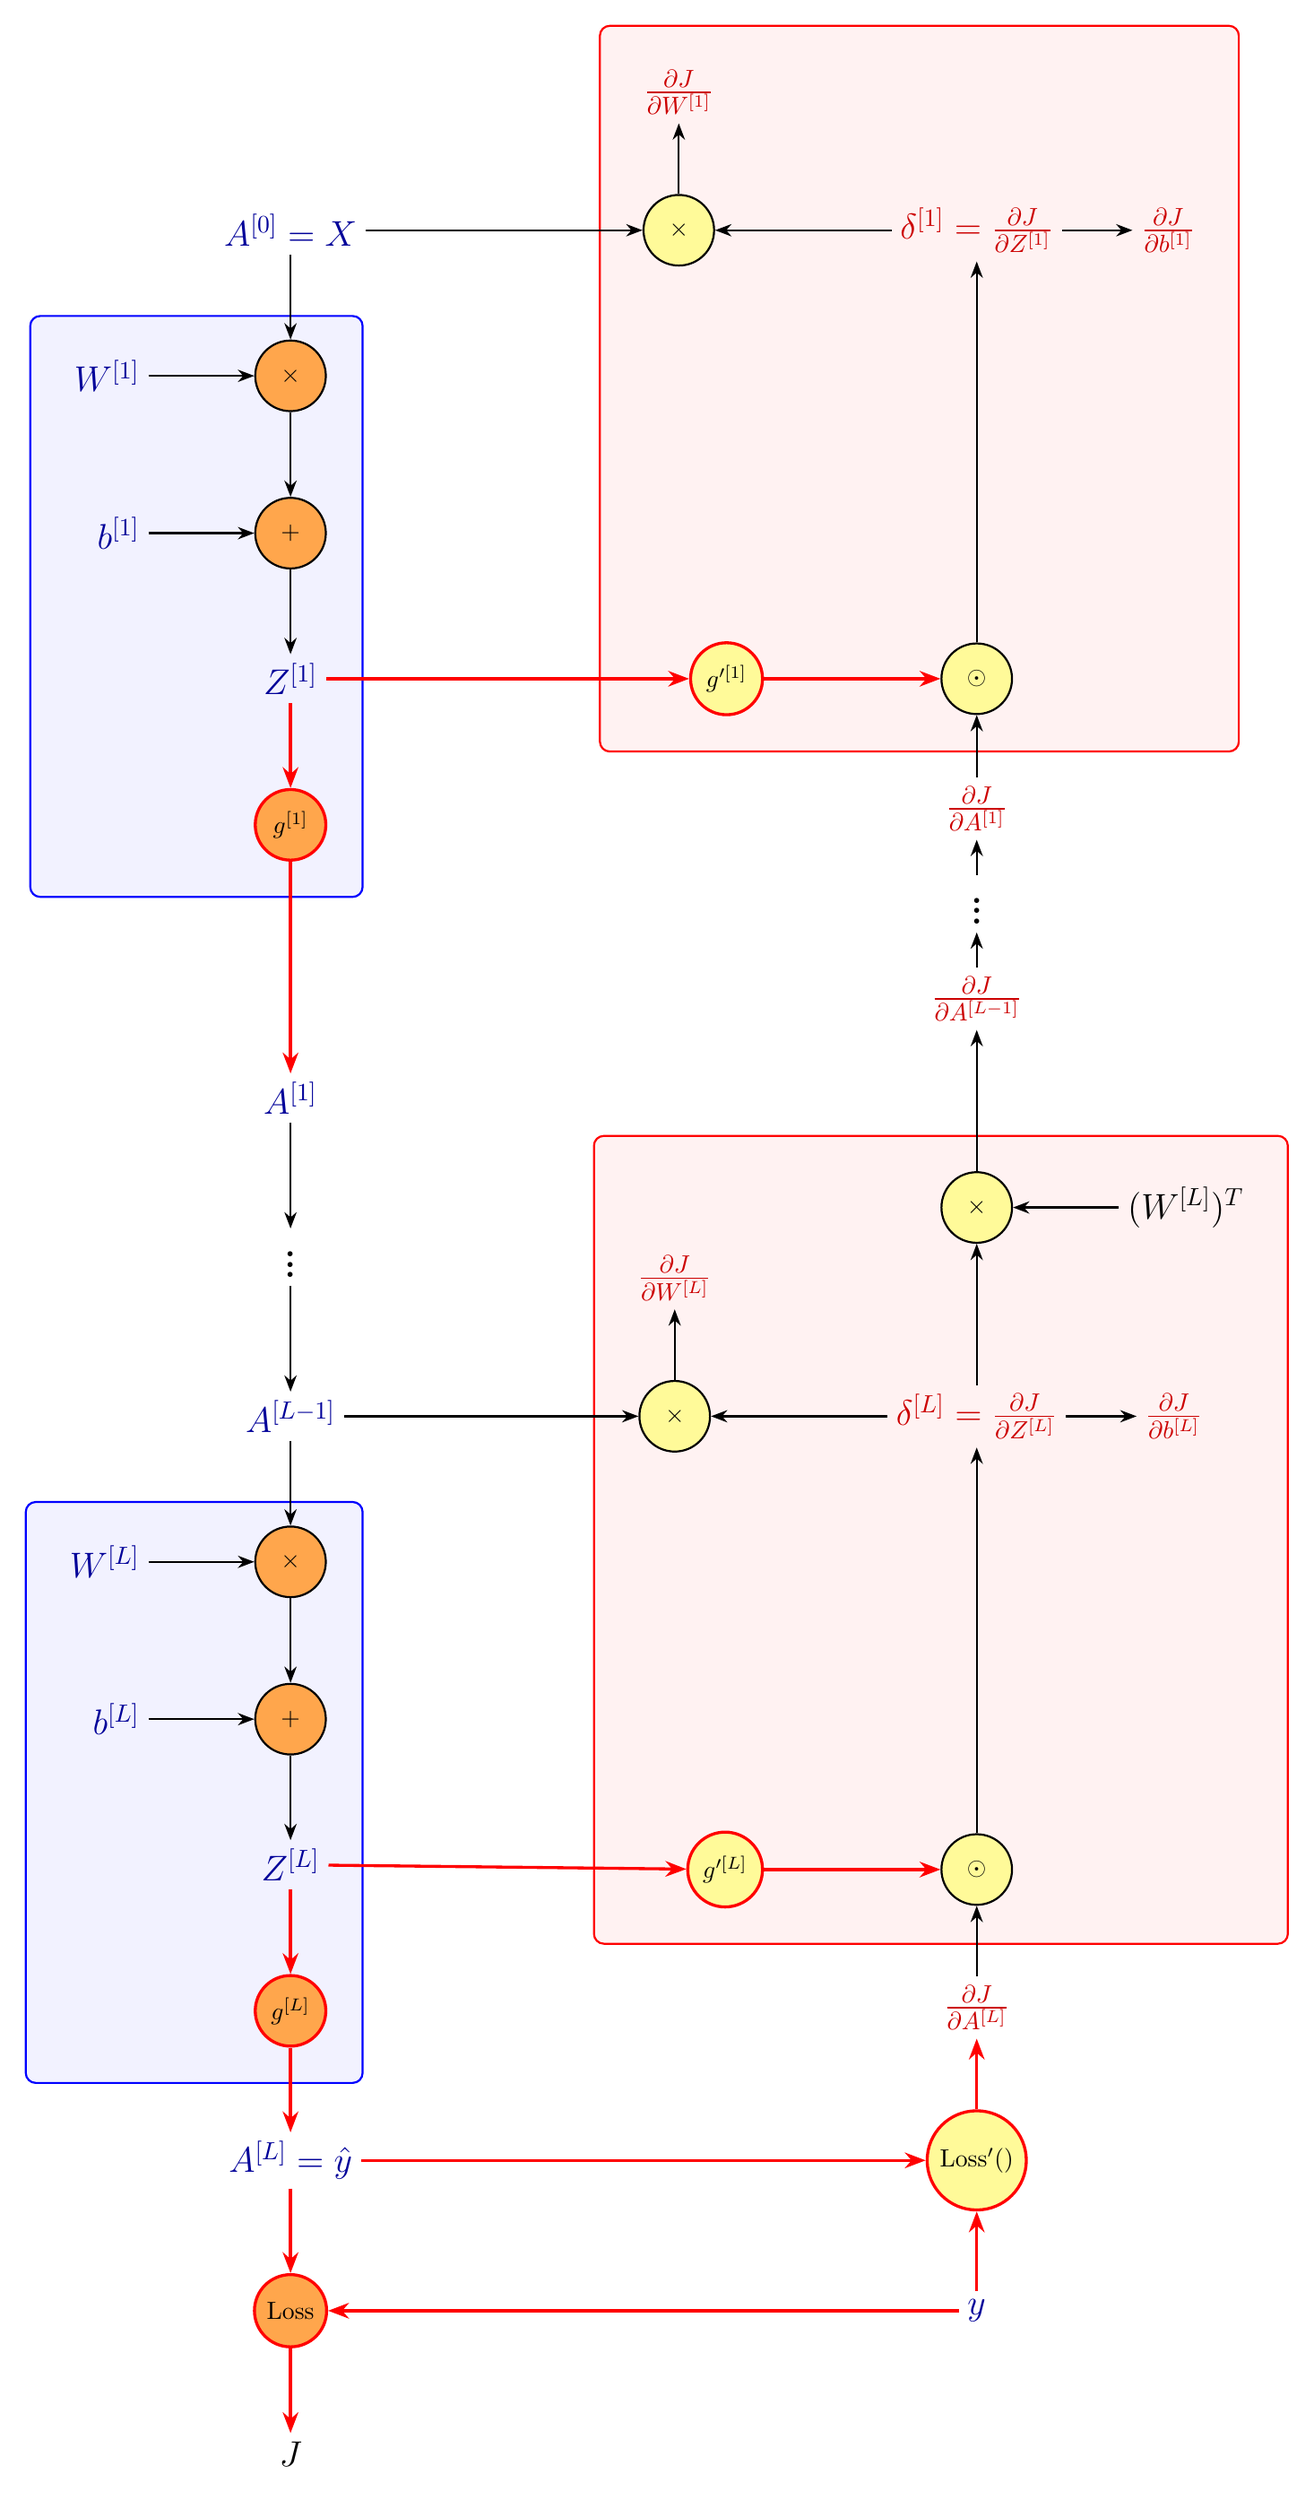
\begin{tikzpicture}[
        node distance=1.5cm and 2.5cm,
        op/.style={circle, draw, thick, minimum size=1cm, fill=yellow!40},
        fwd_op/.style={op, fill=orange!70}, % Style for forward-pass operators
        nonlinear_op/.style={draw=red, very thick}, % Style for non-linear operations
        arrow/.style={Stealth-, thick}, % Arrows flow backwards (B to A in \draw (A)--(B))
        arrow_fwd/.style={-Stealth, thick}, % Arrows for forward pass
        nonlinear_arrow_fwd/.style={arrow_fwd, red, very thick}, % Red arrows for forward non-linear
        nonlinear_arrow_back/.style={arrow, red, very thick}, % Red arrows for backward non-linear
        data/.style={font=\Large},
        grad/.style={font=\Large, text=red!80!black},
        fwd_data/.style={font=\Large, text=blue!60!black},
        layerbox/.style={draw, thick, red, rounded corners, inner sep=0.5cm, fill=red!5},
        fwd_layerbox/.style={draw, thick, blue, rounded corners, inner sep=0.5cm, fill=blue!5}
    ]
    % --- Set up layers to draw boxes in the background ---
    \pgfdeclarelayer{background}
    \pgfsetlayers{background,main}    
    
    \node[fwd_data] (A_0) {$A^{[0]} = X$};
    \node[fwd_op, below = 1.2cm of A_0] (fwd_mult_1) {$\times$};
    \node[fwd_data, left = 1.5cm of fwd_mult_1] (W_1) {$W^{[1]}$};
    \node[fwd_op, below = 1.2cm of fwd_mult_1] (fwd_add_1) {$+$};
    \node[fwd_data, left = 1.5cm of fwd_add_1] (b_1_fwd) {$b^{[1]}$};
    \node[fwd_data, below = 1.2cm of fwd_add_1] (Z_1) {$Z^{[1]}$};

    % Connection from Z_1 to A_1
    \node[fwd_op, nonlinear_op, below = 1.2cm of Z_1] (g_1) {$g^{[1]}$};
    \node[fwd_data, below = 3cm of g_1] (A_1) {$A^{[1]}$};

    % Forward pass dots
    \node[font=\Huge, below = 1.5cm of A_1] (dots_fwd) {$\vdots$};  
    
    % --- Detailed Forward Pass for Layer L ---
    \node[fwd_data, below = 1.5cm of dots_fwd] (A_L_minus_1) {$A^{[L-1]}$};
    \node[fwd_op, below = 1.2cm of A_L_minus_1] (fwd_mult_L) {$\times$};
    \node[fwd_data, left = 1.5cm of fwd_mult_L] (W_L) {$W^{[L]}$};
    \node[fwd_op, below = 1.2cm of fwd_mult_L] (fwd_add_L) {$+$};
    \node[fwd_data, left = 1.5cm of fwd_add_L] (b_L_fwd) {$b^{[L]}$};
    \node[fwd_data, below = 1.2cm of fwd_add_L] (Z_L) {$Z^{[L]}$};
    \node[fwd_op, nonlinear_op, below = 1.2cm of Z_L] (g_L)  {$g^{[L]}$};
    \node[fwd_data, below = 1.2cm of g_L] (y_hat) {$A^{[L]}=\hat{y}$};
    
    % --- Forward Pass Loss Calculation ---
    \node[fwd_op, nonlinear_op, below = 1.2cm of y_hat] (loss_func) {Loss};
    \node[data, below=1.2cm of loss_func] (J) {$J$};    
    
    % --- LOSS FUNCTION (AT THE BOTTOM) ----
    \node[op, nonlinear_op, right = 8cm of y_hat] (loss_prime) {Loss$'$()};    
    \node[fwd_data, at=(loss_prime.south |- loss_func.east)] (y) {$y$};

    % --- LAYER L (ABOVE LOSS) ---
    \node[grad, above = 1cm of loss_prime] (dA_L) {$\frac{\partial J}{\partial A^{[L]}}$};
    \node[op, above = 1cm of dA_L] (had1) {$\odot$};
    \node[op, nonlinear_op, left = 2.5cm of had1] (gprime_L_func) {$g'^{[L]}$};
    \node[grad, at=(had1.north |- A_L_minus_1.east)] (dZ_L) {$\delta^{[L]} = \frac{\partial J}{\partial Z^{[L]}}$};

    \node[op, above = 2cm of dZ_L] (mult_a) {$\times$};
    \node[data, right = 1.5cm of mult_a] (W_L_T) {$(W^{[L]})^T$};
    \node[grad, above = 2cm of mult_a] (dA_L_minus_1) {$\frac{\partial J}{\partial A^{[L-1]}}$};

    \node[op, left = 2.5cm of dZ_L] (mult_w) {$\times$};
    \node[grad, above  = 1cm of mult_w] (dW_L) {$\frac{\partial J}{\partial W^{[L]}}$};
    \node[grad, right = 1cm of dZ_L] (db_L) {$\frac{\partial J}{\partial b^{[L]}}$};

    % --- CONTINUATION DOTS (ABOVE LAYER L) ---
    \node[font=\Huge, above = 0.5cm of dA_L_minus_1] (dots) {$\vdots$};

    % --- LAYER 1 (AT THE TOP) ---
    \node[grad, above = 0.5cm of dots] (dA_1) {$\frac{\partial J}{\partial A^{[1]}}$};
    \node[op, at=(dA_1.north |- Z_1.east)] (had_final) {$\odot$};
    \node[op, nonlinear_op, left = 2.5cm of had_final] (gprime_1_func) {$g'^{[1]}$};
    \node[grad, at=(had_final.north |- A_0.east)] (dZ_1) {$\delta^{[1]} = \frac{\partial J}{\partial Z^{[1]}}$};

    \node[op, left = 2.5cm of dZ_1] (mult_w_final) {$\times$};
    \node[grad, above = 1cm of mult_w_final] (dW_1) {$\frac{\partial J}{\partial W^{[1]}}$};
    \node[grad, right = 1cm of dZ_1] (db_1) {$\frac{\partial J}{\partial b^{[1]}}$};

    % --- ARROWS ---
    % Forward Pass Arrows
    \draw[nonlinear_arrow_fwd] (y_hat) -- (loss_func);
    \draw[nonlinear_arrow_fwd] (y) -- (loss_func);
    \draw[nonlinear_arrow_fwd] (loss_func) -- (J);
    \draw[nonlinear_arrow_fwd] (Z_L) -- (g_L);
    \draw[nonlinear_arrow_fwd] (g_L) -- (y_hat);
    \draw[arrow_fwd] (A_L_minus_1) -- (fwd_mult_L);
    \draw[arrow_fwd] (W_L) -- (fwd_mult_L);
    \draw[arrow_fwd] (fwd_mult_L) -- (fwd_add_L);
    \draw[arrow_fwd] (b_L_fwd) -- (fwd_add_L);
    \draw[arrow_fwd] (fwd_add_L) -- (Z_L);
    \draw[arrow_fwd] (A_0) -- (fwd_mult_1);
    \draw[arrow_fwd] (W_1) -- (fwd_mult_1);
    \draw[arrow_fwd] (fwd_mult_1) -- (fwd_add_1);
    \draw[arrow_fwd] (b_1_fwd) -- (fwd_add_1);
    \draw[arrow_fwd] (fwd_add_1) -- (Z_1);
    \draw[nonlinear_arrow_fwd] (Z_1) -- (g_1);
    \draw[nonlinear_arrow_fwd] (g_1) -- (A_1);
    \draw[arrow_fwd] (A_1) -- (dots_fwd);
    \draw[arrow_fwd] (dots_fwd) -- (A_L_minus_1);

    % Backpropagation Arrows
    \draw[nonlinear_arrow_back] (loss_prime) -- (y_hat);
    \draw[nonlinear_arrow_back] (loss_prime) -- (y);
    \draw[nonlinear_arrow_back] (dA_L) -- (loss_prime);
    \draw[arrow] (had1) -- (dA_L);
    \draw[nonlinear_arrow_back] (had1) -- (gprime_L_func);
    \draw[nonlinear_arrow_back] (gprime_L_func) -- (Z_L);
    \draw[arrow] (dZ_L) -- (had1);
    \draw[arrow] (mult_w) -- (dZ_L);
    \draw[arrow] (mult_w) -- (A_L_minus_1);
    \draw[arrow] (dW_L) -- (mult_w);
    \draw[arrow] (db_L) -- (dZ_L);
    \draw[arrow] (mult_a) -- (dZ_L);
    \draw[arrow] (mult_a) -- (W_L_T);
    \draw[arrow] (dA_L_minus_1) -- (mult_a);
    \draw[arrow] (dots) -- (dA_L_minus_1);
    \draw[arrow] (dA_1) -- (dots);
    \draw[arrow] (had_final) -- (dA_1);
    \draw[nonlinear_arrow_back] (had_final) -- (gprime_1_func);
    \draw[nonlinear_arrow_back] (gprime_1_func) -- (Z_1);
    \draw[arrow] (dZ_1) -- (had_final);
    \draw[arrow] (mult_w_final) -- (dZ_1);
    \draw[arrow] (mult_w_final) -- (A_0);
    \draw[arrow] (dW_1) -- (mult_w_final);
    \draw[arrow] (db_1) -- (dZ_1);

\begin{pgfonlayer}{background}
    % Box for Layer L (Backpropagation)
    \node[layerbox,
          fit=(gprime_L_func) (had1) (dZ_L) (mult_a) (W_L_T) (dW_L) (db_L) ] {};
    % Box for Layer 1 (Backpropagation)
    \node[layerbox,
          fit=(gprime_1_func) (had_final) (dZ_1) (mult_w_final) (dW_1) (db_1)] {};
    % New box for Layer L (Forward Pass)
    \node[fwd_layerbox,
          fit=(W_L) (g_L)] {};
    % New box for Layer 1 (Forward Pass)
    \node[fwd_layerbox,
          fit=(W_1) (g_1)] {};
\end{pgfonlayer}

    \end{tikzpicture}%
}

\ifdefined\ispartofbook
  % This part is intentionally left blank when included in the main book.
  % The \newcommand is defined, and the chapter file is responsible for calling it.
\else
  % This part is for standalone compilation of the image.
  \combineddiagram 
  \end{document}
\fi
 % For standalone compilation
  % This file defines the command for the combined forward/backward pass diagram.
% It can be compiled standalone or included in a larger document.

\ifdefined\ispartofbook
\else
  % --- Standalone Compilation Preamble ---
  \documentclass[tikz, border=10pt]{standalone}
  \usepackage{amsmath, amssymb} % For math symbols
  \usepackage{tikz}
  \usetikzlibrary{
    positioning,
    arrows.meta,
    fit,
    decorations.pathreplacing,
    calligraphy,
    shapes.geometric,
    shadows,
    chains,
    backgrounds
  }
  \begin{document}
\fi

% --- THE DIAGRAM COMMAND ---
\newcommand{\combineddiagram}{%
    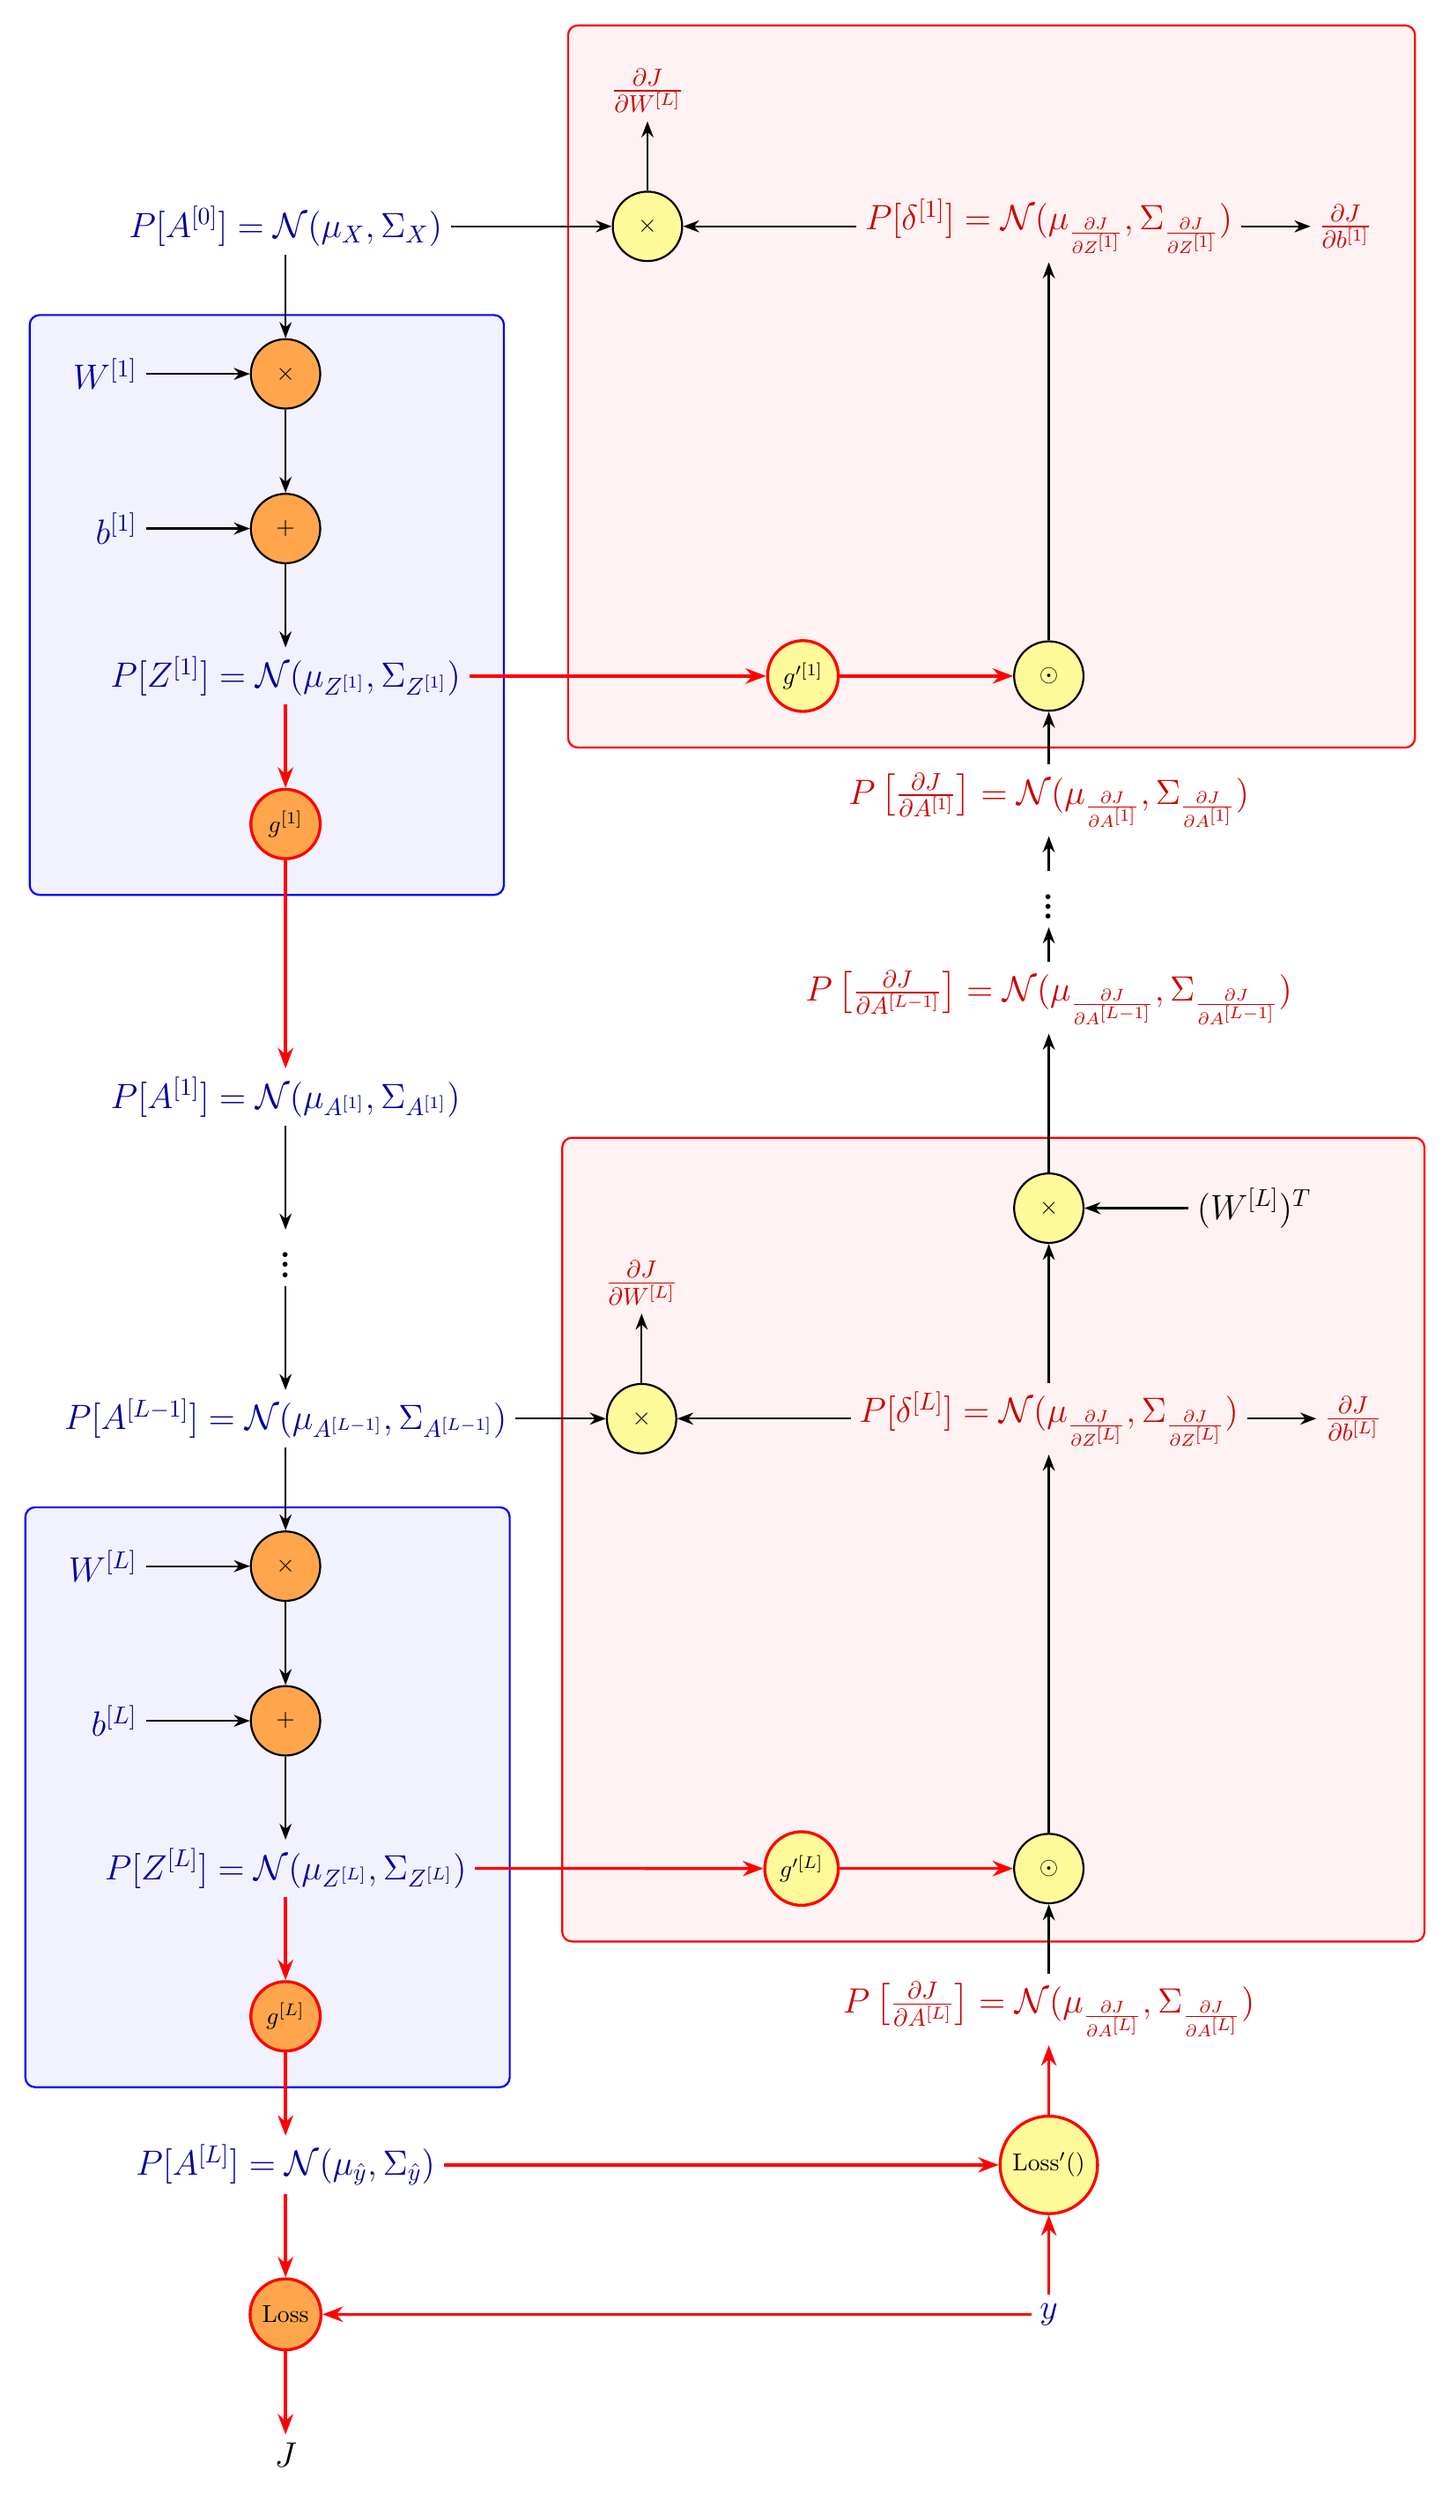
\begin{tikzpicture}[
        node distance=1.5cm and 2.5cm,
        op/.style={circle, draw, thick, minimum size=1cm, fill=yellow!40},
        fwd_op/.style={op, fill=orange!70}, % Style for forward-pass operators
        nonlinear_op/.style={draw=red, very thick}, % Style for non-linear operations
        arrow/.style={Stealth-, thick}, % Arrows flow backwards (B to A in \draw (A)--(B))
        arrow_fwd/.style={-Stealth, thick}, % Arrows for forward pass
        nonlinear_arrow_fwd/.style={arrow_fwd, red, very thick}, % Red arrows for forward non-linear
        nonlinear_arrow_back/.style={arrow, red, very thick}, % Red arrows for backward non-linear
        data/.style={font=\Large},
        grad/.style={font=\Large, text=red!80!black},
        fwd_data/.style={font=\Large, text=blue!60!black},
        layerbox/.style={draw, thick, red, rounded corners, inner sep=0.5cm, fill=red!5},
        fwd_layerbox/.style={draw, thick, blue, rounded corners, inner sep=0.5cm, fill=blue!5}
    ]
    % --- Set up layers to draw boxes in the background ---
    \pgfdeclarelayer{background}
    \pgfsetlayers{background,main}    
    
    \node[fwd_data] (A_0) {$P[A^{[0]}] = \mathcal{N}(\mu_X, \Sigma_X)$};
    \node[fwd_op, below = 1.2cm of A_0] (fwd_mult_1) {$\times$};
    \node[fwd_data, left = 1.5cm of fwd_mult_1] (W_1) {$W^{[1]}$};
    \node[fwd_op, below = 1.2cm of fwd_mult_1] (fwd_add_1) {$+$};
    \node[fwd_data, left = 1.5cm of fwd_add_1] (b_1_fwd) {$b^{[1]}$};
    \node[fwd_data, below = 1.2cm of fwd_add_1] (Z_1) {$P[Z^{[1]}] = \mathcal{N}(\mu_{Z^{[1]}}, \Sigma_{Z^{[1]}})$};

    % Connection from Z_1 to A_1
    \node[fwd_op, nonlinear_op, below = 1.2cm of Z_1] (g_1) {$g^{[1]}$};
    \node[fwd_data, below = 3cm of g_1] (A_1) {$P[A^{[1]}] = \mathcal{N}(\mu_{A^{[1]}}, \Sigma_{A^{[1]}})$};

    % Forward pass dots
    \node[font=\Huge, below = 1.5cm of A_1] (dots_fwd) {$\vdots$};  
    
    % --- Detailed Forward Pass for Layer L ---
    \node[fwd_data, below = 1.5cm of dots_fwd] (A_L_minus_1) {$P[A^{[L-1]}] = \mathcal{N}(\mu_{A^{[L-1]}}, \Sigma_{A^{[L-1]}})$};
    \node[fwd_op, below = 1.2cm of A_L_minus_1] (fwd_mult_L) {$\times$};
    \node[fwd_data, left = 1.5cm of fwd_mult_L] (W_L) {$W^{[L]}$};
    \node[fwd_op, below = 1.2cm of fwd_mult_L] (fwd_add_L) {$+$};
    \node[fwd_data, left = 1.5cm of fwd_add_L] (b_L_fwd) {$b^{[L]}$};
    \node[fwd_data, below = 1.2cm of fwd_add_L] (Z_L) {$P[Z^{[L]}] = \mathcal{N}(\mu_{Z^{[L]}}, \Sigma_{Z^{[L]}})$};
    \node[fwd_op, nonlinear_op, below = 1.2cm of Z_L] (g_L)  {$g^{[L]}$};
    \node[fwd_data, below = 1.2cm of g_L] (y_hat) {$P[A^{[L]}] = \mathcal{N}(\mu_{\hat{y}}, \Sigma_{\hat{y}})$};
    
    % --- Forward Pass Loss Calculation ---
    \node[fwd_op, nonlinear_op, below = 1.2cm of y_hat] (loss_func) {Loss};
    \node[data, below=1.2cm of loss_func] (J) {$J$};    
    
    % --- LOSS FUNCTION (AT THE BOTTOM) ----
    \node[op, nonlinear_op, right = 8cm of y_hat] (loss_prime) {Loss$'$()};    
    \node[fwd_data, at=(loss_prime.south |- loss_func.east)] (y) {$y$};

    % --- LAYER L (ABOVE LOSS) ---
    \node[grad, above = 1cm of loss_prime] (dA_L) {$P\left[\frac{\partial J}{\partial A^{[L]}}\right] = \mathcal{N}(\mu_{\frac{\partial J}{\partial A^{[L]}}}, \Sigma_{\frac{\partial J}{\partial A^{[L]}}})$};
    \node[op, above = 1cm of dA_L] (had1) {$\odot$};
    \node[op, nonlinear_op, left = 2.5cm of had1] (gprime_L_func) {$g'^{[L]}$};
    \node[grad, at=(had1.north |- A_L_minus_1.east)] (dZ_L) {$P[\delta^{[L]}] = \mathcal{N}(\mu_{\frac{\partial J}{\partial Z^{[L]}}}, \Sigma_{\frac{\partial J}{\partial Z^{[L]}}})$};

    \node[op, above = 2cm of dZ_L] (mult_a) {$\times$};
    \node[data, right = 1.5cm of mult_a] (W_L_T) {$(W^{[L]})^T$};
    \node[grad, above = 2cm of mult_a] (dA_L_minus_1) {$P\left[\frac{\partial J}{\partial A^{[L-1]}}\right] = \mathcal{N}(\mu_{\frac{\partial J}{\partial A^{[L-1]}}}, \Sigma_{\frac{\partial J}{\partial A^{[L-1]}}})$};

    \node[op, left = 2.5cm of dZ_L] (mult_w) {$\times$};
    \node[grad, above  = 1cm of mult_w] (dW_L) {$\frac{\partial J}{\partial W^{[L]}}$};
    \node[grad, right = 1cm of dZ_L] (db_L) {$\frac{\partial J}{\partial b^{[L]}}$};

    % --- CONTINUATION DOTS (ABOVE LAYER L) ---
    \node[font=\Huge, above = 0.5cm of dA_L_minus_1] (dots) {$\vdots$};

    % --- LAYER 1 (AT THE TOP) ---
    \node[grad, above = 0.5cm of dots] (dA_1) {$P\left[\frac{\partial J}{\partial A^{[1]}}\right] = \mathcal{N}(\mu_{\frac{\partial J}{\partial A^{[1]}}}, \Sigma_{\frac{\partial J}{\partial A^{[1]}}})$};
    \node[op, at=(dA_1.north |- Z_1.east)] (had_final) {$\odot$};
    \node[op, nonlinear_op, left = 2.5cm of had_final] (gprime_1_func) {$g'^{[1]}$};
    \node[grad, at=(had_final.north |- A_0.east)] (dZ_1) {$P[\delta^{[1]}] = \mathcal{N}(\mu_{\frac{\partial J}{\partial Z^{[1]}}}, \Sigma_{\frac{\partial J}{\partial Z^{[1]}}})$};

    \node[op, left = 2.5cm of dZ_1] (mult_w_final) {$\times$};
    \node[grad, above = 1cm of mult_w_final] (dW_1) {$\frac{\partial J}{\partial W^{[L]}}$};
    \node[grad, right = 1cm of dZ_1] (db_1) {$\frac{\partial J}{\partial b^{[1]}}$};

    % --- ARROWS ---
    % Forward Pass Arrows
    \draw[nonlinear_arrow_fwd] (y_hat) -- (loss_func);
    \draw[nonlinear_arrow_fwd] (y) -- (loss_func);
    \draw[nonlinear_arrow_fwd] (loss_func) -- (J);
    \draw[nonlinear_arrow_fwd] (Z_L) -- (g_L);
    \draw[nonlinear_arrow_fwd] (g_L) -- (y_hat);
    \draw[arrow_fwd] (A_L_minus_1) -- (fwd_mult_L);
    \draw[arrow_fwd] (W_L) -- (fwd_mult_L);
    \draw[arrow_fwd] (fwd_mult_L) -- (fwd_add_L);
    \draw[arrow_fwd] (b_L_fwd) -- (fwd_add_L);
    \draw[arrow_fwd] (fwd_add_L) -- (Z_L);
    \draw[arrow_fwd] (A_0) -- (fwd_mult_1);
    \draw[arrow_fwd] (W_1) -- (fwd_mult_1);
    \draw[arrow_fwd] (fwd_mult_1) -- (fwd_add_1);
    \draw[arrow_fwd] (b_1_fwd) -- (fwd_add_1);
    \draw[arrow_fwd] (fwd_add_1) -- (Z_1);
    \draw[nonlinear_arrow_fwd] (Z_1) -- (g_1);
    \draw[nonlinear_arrow_fwd] (g_1) -- (A_1);
    \draw[arrow_fwd] (A_1) -- (dots_fwd);
    \draw[arrow_fwd] (dots_fwd) -- (A_L_minus_1);

    % Backpropagation Arrows
    \draw[nonlinear_arrow_back] (loss_prime) -- (y_hat);
    \draw[nonlinear_arrow_back] (loss_prime) -- (y);
    \draw[nonlinear_arrow_back] (dA_L) -- (loss_prime);
    \draw[arrow] (had1) -- (dA_L);
    \draw[nonlinear_arrow_back] (had1) -- (gprime_L_func);
    \draw[nonlinear_arrow_back] (gprime_L_func) -- (Z_L);
    \draw[arrow] (dZ_L) -- (had1);
    \draw[arrow] (mult_w) -- (dZ_L);
    \draw[arrow] (mult_w) -- (A_L_minus_1);
    \draw[arrow] (dW_L) -- (mult_w);
    \draw[arrow] (db_L) -- (dZ_L);
    \draw[arrow] (mult_a) -- (dZ_L);
    \draw[arrow] (mult_a) -- (W_L_T);
    \draw[arrow] (dA_L_minus_1) -- (mult_a);
    \draw[arrow] (dots) -- (dA_L_minus_1);
    \draw[arrow] (dA_1) -- (dots);
    \draw[arrow] (had_final) -- (dA_1);
    \draw[nonlinear_arrow_back] (had_final) -- (gprime_1_func);
    \draw[nonlinear_arrow_back] (gprime_1_func) -- (Z_1);
    \draw[arrow] (dZ_1) -- (had_final);
    \draw[arrow] (mult_w_final) -- (dZ_1);
    \draw[arrow] (mult_w_final) -- (A_0);
    \draw[arrow] (dW_1) -- (mult_w_final);
    \draw[arrow] (db_1) -- (dZ_1);

\begin{pgfonlayer}{background}
    % Box for Layer L (Backpropagation)
    \node[layerbox,
          fit=(gprime_L_func) (had1) (dZ_L) (mult_a) (W_L_T) (dW_L) (db_L) ] {};
    % Box for Layer 1 (Backpropagation)
    \node[layerbox,
          fit=(gprime_1_func) (had_final) (dZ_1) (mult_w_final) (dW_1) (db_1)] {};
    % New box for Layer L (Forward Pass)
    \node[fwd_layerbox,
          fit=(W_L) (Z_L) (g_L)] {};
    % New box for Layer 1 (Forward Pass)
    \node[fwd_layerbox,
          fit=(W_1) (Z_1) (g_1)] {};
\end{pgfonlayer}

    \end{tikzpicture}%
}

\ifdefined\ispartofbook
  % This part is intentionally left blank when included in the main book.
  % The \newcommand is defined, and the chapter file is responsible for calling it.
\else
  % This part is for standalone compilation of the image.
  \combineddiagram 
  \end{document}
\fi
 % For standalone compilation
\fi

% This file defines the command for the combined forward/backward pass diagram.
% It can be compiled standalone or included in a larger document.

\ifdefined\ispartofbook
\else
  % --- Standalone Compilation Preamble ---
  \documentclass[tikz, border=10pt]{standalone}
  \usepackage{amsmath, amssymb} % For math symbols
  \usepackage{tikz}
  \usetikzlibrary{
    positioning,
    arrows.meta,
    fit,
    decorations.pathreplacing,
    calligraphy,
    shapes.geometric,
    shadows,
    chains,
    backgrounds
  }
  \begin{document}
\fi

% --- THE DIAGRAM COMMAND ---
\newcommand{\combineddiagram}{%
    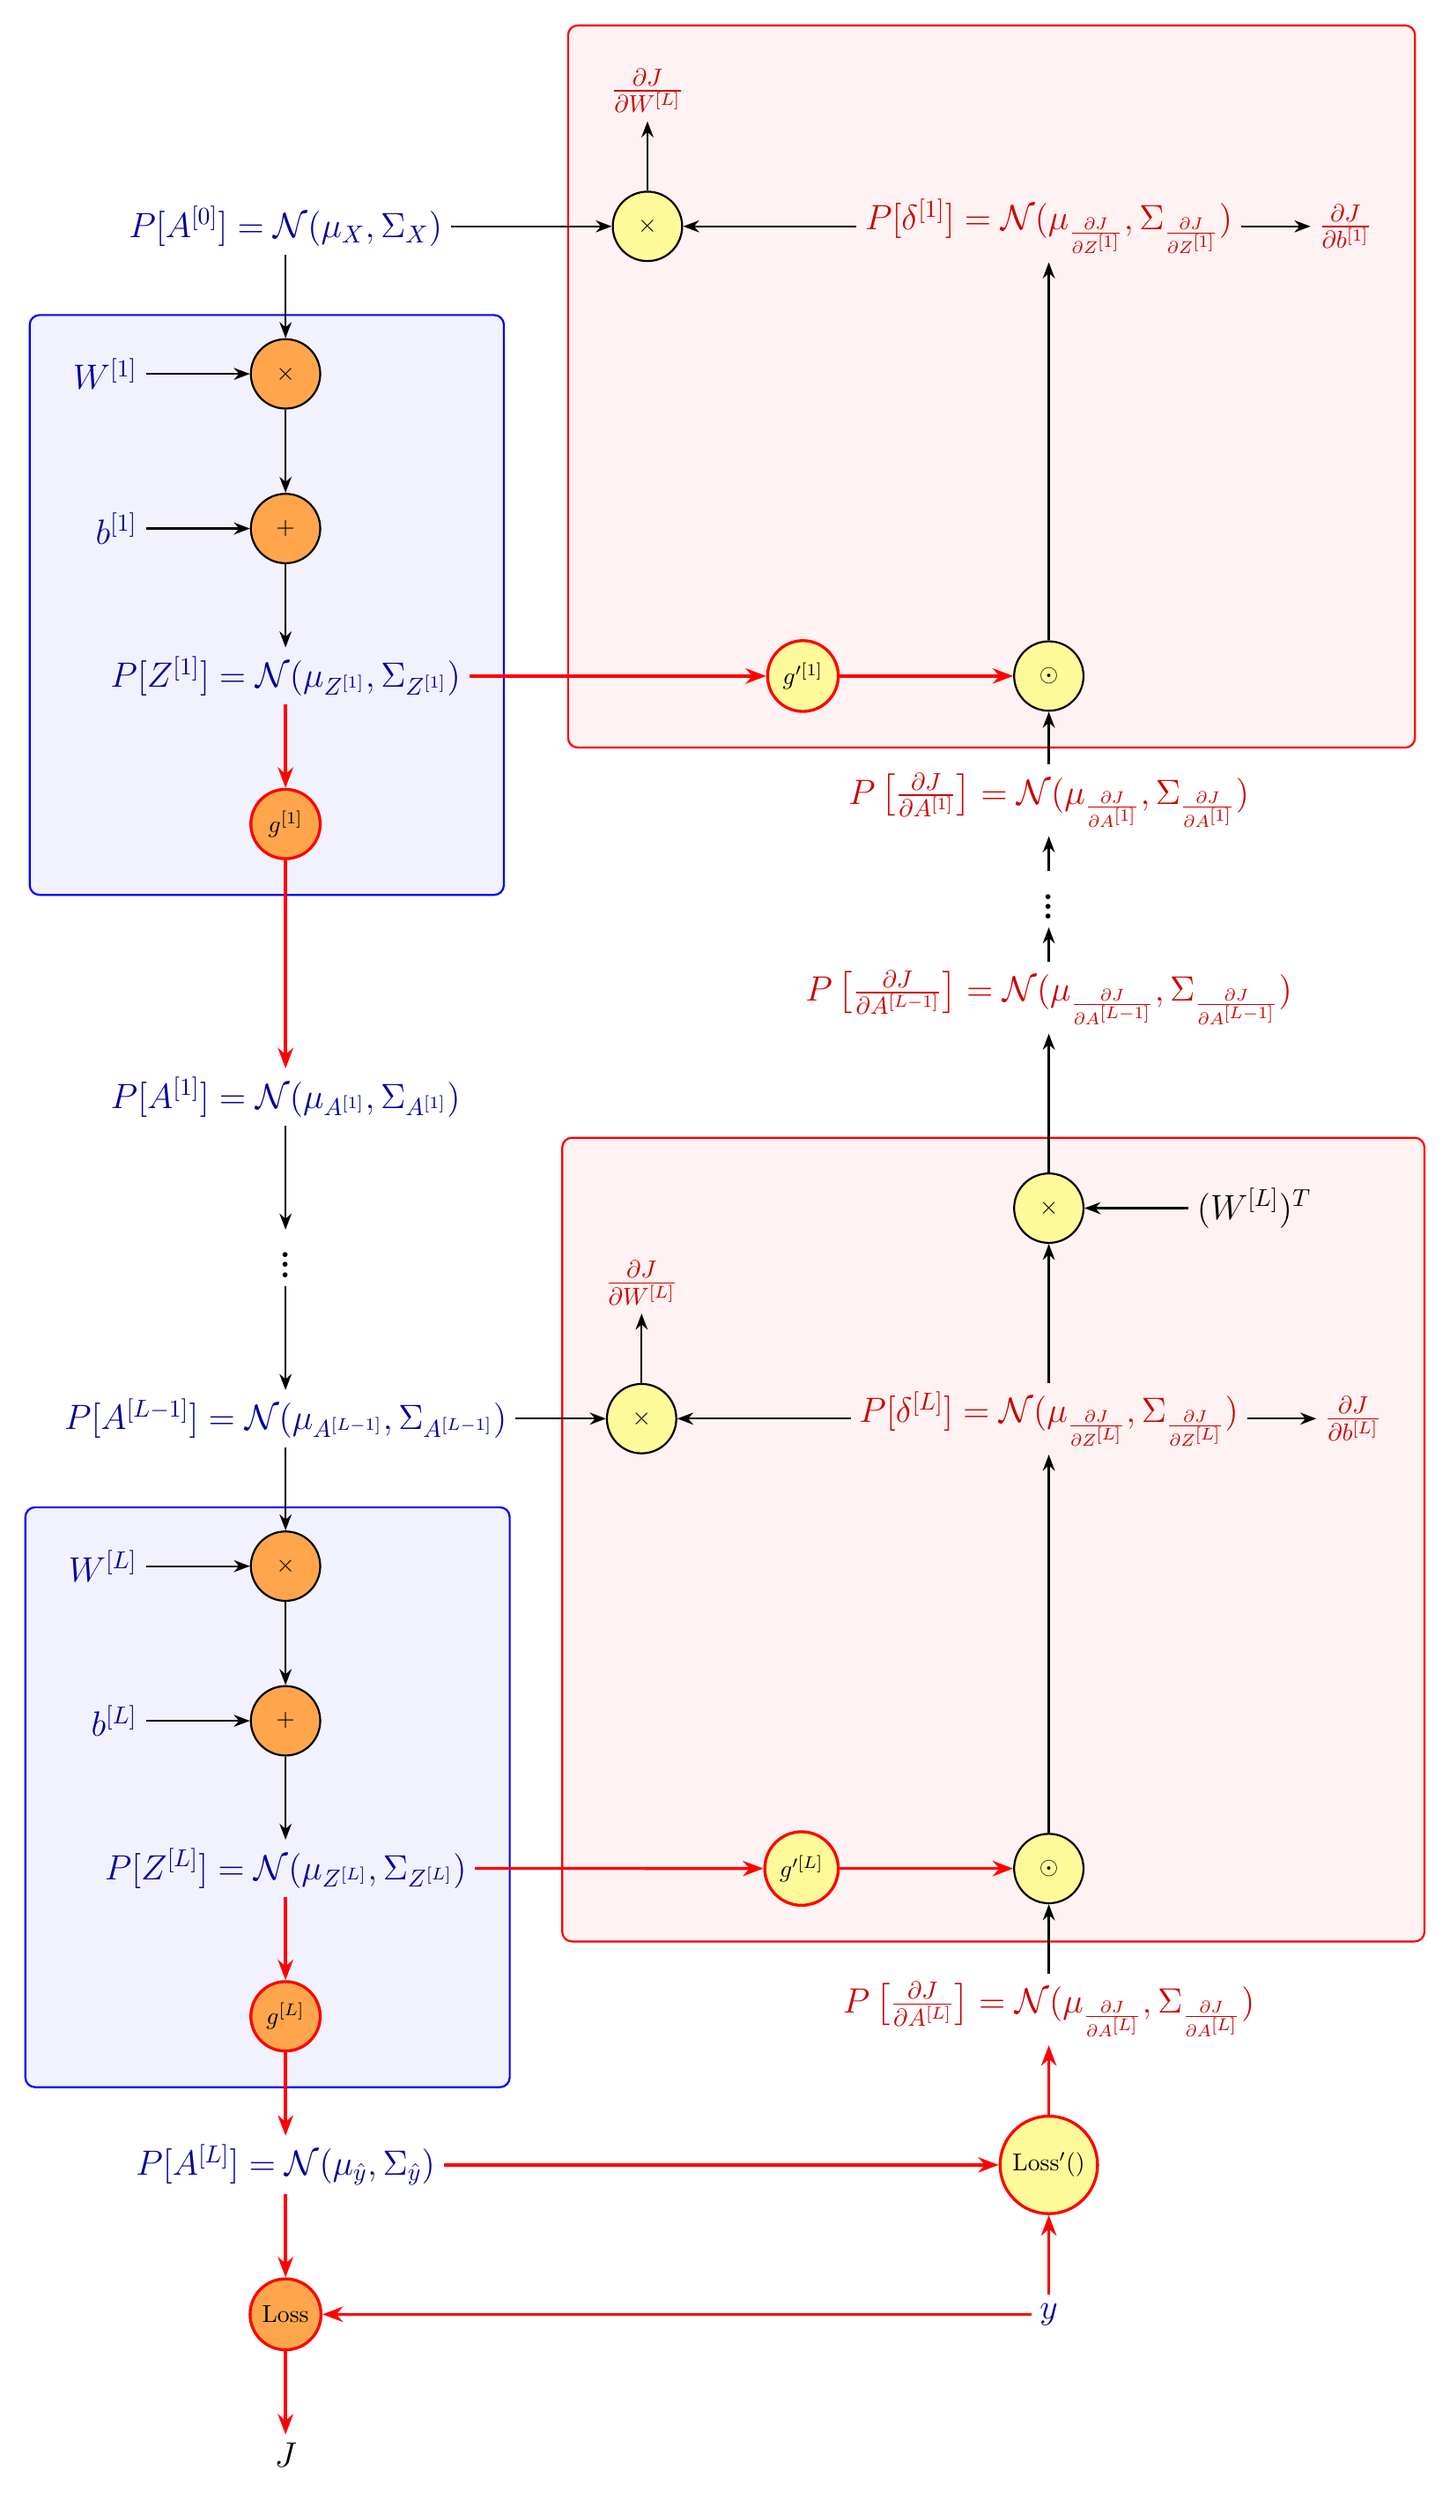
\begin{tikzpicture}[
        node distance=1.5cm and 2.5cm,
        op/.style={circle, draw, thick, minimum size=1cm, fill=yellow!40},
        fwd_op/.style={op, fill=orange!70}, % Style for forward-pass operators
        nonlinear_op/.style={draw=red, very thick}, % Style for non-linear operations
        arrow/.style={Stealth-, thick}, % Arrows flow backwards (B to A in \draw (A)--(B))
        arrow_fwd/.style={-Stealth, thick}, % Arrows for forward pass
        nonlinear_arrow_fwd/.style={arrow_fwd, red, very thick}, % Red arrows for forward non-linear
        nonlinear_arrow_back/.style={arrow, red, very thick}, % Red arrows for backward non-linear
        data/.style={font=\Large},
        grad/.style={font=\Large, text=red!80!black},
        fwd_data/.style={font=\Large, text=blue!60!black},
        layerbox/.style={draw, thick, red, rounded corners, inner sep=0.5cm, fill=red!5},
        fwd_layerbox/.style={draw, thick, blue, rounded corners, inner sep=0.5cm, fill=blue!5}
    ]
    % --- Set up layers to draw boxes in the background ---
    \pgfdeclarelayer{background}
    \pgfsetlayers{background,main}    
    
    \node[fwd_data] (A_0) {$P[A^{[0]}] = \mathcal{N}(\mu_X, \Sigma_X)$};
    \node[fwd_op, below = 1.2cm of A_0] (fwd_mult_1) {$\times$};
    \node[fwd_data, left = 1.5cm of fwd_mult_1] (W_1) {$W^{[1]}$};
    \node[fwd_op, below = 1.2cm of fwd_mult_1] (fwd_add_1) {$+$};
    \node[fwd_data, left = 1.5cm of fwd_add_1] (b_1_fwd) {$b^{[1]}$};
    \node[fwd_data, below = 1.2cm of fwd_add_1] (Z_1) {$P[Z^{[1]}] = \mathcal{N}(\mu_{Z^{[1]}}, \Sigma_{Z^{[1]}})$};

    % Connection from Z_1 to A_1
    \node[fwd_op, nonlinear_op, below = 1.2cm of Z_1] (g_1) {$g^{[1]}$};
    \node[fwd_data, below = 3cm of g_1] (A_1) {$P[A^{[1]}] = \mathcal{N}(\mu_{A^{[1]}}, \Sigma_{A^{[1]}})$};

    % Forward pass dots
    \node[font=\Huge, below = 1.5cm of A_1] (dots_fwd) {$\vdots$};  
    
    % --- Detailed Forward Pass for Layer L ---
    \node[fwd_data, below = 1.5cm of dots_fwd] (A_L_minus_1) {$P[A^{[L-1]}] = \mathcal{N}(\mu_{A^{[L-1]}}, \Sigma_{A^{[L-1]}})$};
    \node[fwd_op, below = 1.2cm of A_L_minus_1] (fwd_mult_L) {$\times$};
    \node[fwd_data, left = 1.5cm of fwd_mult_L] (W_L) {$W^{[L]}$};
    \node[fwd_op, below = 1.2cm of fwd_mult_L] (fwd_add_L) {$+$};
    \node[fwd_data, left = 1.5cm of fwd_add_L] (b_L_fwd) {$b^{[L]}$};
    \node[fwd_data, below = 1.2cm of fwd_add_L] (Z_L) {$P[Z^{[L]}] = \mathcal{N}(\mu_{Z^{[L]}}, \Sigma_{Z^{[L]}})$};
    \node[fwd_op, nonlinear_op, below = 1.2cm of Z_L] (g_L)  {$g^{[L]}$};
    \node[fwd_data, below = 1.2cm of g_L] (y_hat) {$P[A^{[L]}] = \mathcal{N}(\mu_{\hat{y}}, \Sigma_{\hat{y}})$};
    
    % --- Forward Pass Loss Calculation ---
    \node[fwd_op, nonlinear_op, below = 1.2cm of y_hat] (loss_func) {Loss};
    \node[data, below=1.2cm of loss_func] (J) {$J$};    
    
    % --- LOSS FUNCTION (AT THE BOTTOM) ----
    \node[op, nonlinear_op, right = 8cm of y_hat] (loss_prime) {Loss$'$()};    
    \node[fwd_data, at=(loss_prime.south |- loss_func.east)] (y) {$y$};

    % --- LAYER L (ABOVE LOSS) ---
    \node[grad, above = 1cm of loss_prime] (dA_L) {$P\left[\frac{\partial J}{\partial A^{[L]}}\right] = \mathcal{N}(\mu_{\frac{\partial J}{\partial A^{[L]}}}, \Sigma_{\frac{\partial J}{\partial A^{[L]}}})$};
    \node[op, above = 1cm of dA_L] (had1) {$\odot$};
    \node[op, nonlinear_op, left = 2.5cm of had1] (gprime_L_func) {$g'^{[L]}$};
    \node[grad, at=(had1.north |- A_L_minus_1.east)] (dZ_L) {$P[\delta^{[L]}] = \mathcal{N}(\mu_{\frac{\partial J}{\partial Z^{[L]}}}, \Sigma_{\frac{\partial J}{\partial Z^{[L]}}})$};

    \node[op, above = 2cm of dZ_L] (mult_a) {$\times$};
    \node[data, right = 1.5cm of mult_a] (W_L_T) {$(W^{[L]})^T$};
    \node[grad, above = 2cm of mult_a] (dA_L_minus_1) {$P\left[\frac{\partial J}{\partial A^{[L-1]}}\right] = \mathcal{N}(\mu_{\frac{\partial J}{\partial A^{[L-1]}}}, \Sigma_{\frac{\partial J}{\partial A^{[L-1]}}})$};

    \node[op, left = 2.5cm of dZ_L] (mult_w) {$\times$};
    \node[grad, above  = 1cm of mult_w] (dW_L) {$\frac{\partial J}{\partial W^{[L]}}$};
    \node[grad, right = 1cm of dZ_L] (db_L) {$\frac{\partial J}{\partial b^{[L]}}$};

    % --- CONTINUATION DOTS (ABOVE LAYER L) ---
    \node[font=\Huge, above = 0.5cm of dA_L_minus_1] (dots) {$\vdots$};

    % --- LAYER 1 (AT THE TOP) ---
    \node[grad, above = 0.5cm of dots] (dA_1) {$P\left[\frac{\partial J}{\partial A^{[1]}}\right] = \mathcal{N}(\mu_{\frac{\partial J}{\partial A^{[1]}}}, \Sigma_{\frac{\partial J}{\partial A^{[1]}}})$};
    \node[op, at=(dA_1.north |- Z_1.east)] (had_final) {$\odot$};
    \node[op, nonlinear_op, left = 2.5cm of had_final] (gprime_1_func) {$g'^{[1]}$};
    \node[grad, at=(had_final.north |- A_0.east)] (dZ_1) {$P[\delta^{[1]}] = \mathcal{N}(\mu_{\frac{\partial J}{\partial Z^{[1]}}}, \Sigma_{\frac{\partial J}{\partial Z^{[1]}}})$};

    \node[op, left = 2.5cm of dZ_1] (mult_w_final) {$\times$};
    \node[grad, above = 1cm of mult_w_final] (dW_1) {$\frac{\partial J}{\partial W^{[L]}}$};
    \node[grad, right = 1cm of dZ_1] (db_1) {$\frac{\partial J}{\partial b^{[1]}}$};

    % --- ARROWS ---
    % Forward Pass Arrows
    \draw[nonlinear_arrow_fwd] (y_hat) -- (loss_func);
    \draw[nonlinear_arrow_fwd] (y) -- (loss_func);
    \draw[nonlinear_arrow_fwd] (loss_func) -- (J);
    \draw[nonlinear_arrow_fwd] (Z_L) -- (g_L);
    \draw[nonlinear_arrow_fwd] (g_L) -- (y_hat);
    \draw[arrow_fwd] (A_L_minus_1) -- (fwd_mult_L);
    \draw[arrow_fwd] (W_L) -- (fwd_mult_L);
    \draw[arrow_fwd] (fwd_mult_L) -- (fwd_add_L);
    \draw[arrow_fwd] (b_L_fwd) -- (fwd_add_L);
    \draw[arrow_fwd] (fwd_add_L) -- (Z_L);
    \draw[arrow_fwd] (A_0) -- (fwd_mult_1);
    \draw[arrow_fwd] (W_1) -- (fwd_mult_1);
    \draw[arrow_fwd] (fwd_mult_1) -- (fwd_add_1);
    \draw[arrow_fwd] (b_1_fwd) -- (fwd_add_1);
    \draw[arrow_fwd] (fwd_add_1) -- (Z_1);
    \draw[nonlinear_arrow_fwd] (Z_1) -- (g_1);
    \draw[nonlinear_arrow_fwd] (g_1) -- (A_1);
    \draw[arrow_fwd] (A_1) -- (dots_fwd);
    \draw[arrow_fwd] (dots_fwd) -- (A_L_minus_1);

    % Backpropagation Arrows
    \draw[nonlinear_arrow_back] (loss_prime) -- (y_hat);
    \draw[nonlinear_arrow_back] (loss_prime) -- (y);
    \draw[nonlinear_arrow_back] (dA_L) -- (loss_prime);
    \draw[arrow] (had1) -- (dA_L);
    \draw[nonlinear_arrow_back] (had1) -- (gprime_L_func);
    \draw[nonlinear_arrow_back] (gprime_L_func) -- (Z_L);
    \draw[arrow] (dZ_L) -- (had1);
    \draw[arrow] (mult_w) -- (dZ_L);
    \draw[arrow] (mult_w) -- (A_L_minus_1);
    \draw[arrow] (dW_L) -- (mult_w);
    \draw[arrow] (db_L) -- (dZ_L);
    \draw[arrow] (mult_a) -- (dZ_L);
    \draw[arrow] (mult_a) -- (W_L_T);
    \draw[arrow] (dA_L_minus_1) -- (mult_a);
    \draw[arrow] (dots) -- (dA_L_minus_1);
    \draw[arrow] (dA_1) -- (dots);
    \draw[arrow] (had_final) -- (dA_1);
    \draw[nonlinear_arrow_back] (had_final) -- (gprime_1_func);
    \draw[nonlinear_arrow_back] (gprime_1_func) -- (Z_1);
    \draw[arrow] (dZ_1) -- (had_final);
    \draw[arrow] (mult_w_final) -- (dZ_1);
    \draw[arrow] (mult_w_final) -- (A_0);
    \draw[arrow] (dW_1) -- (mult_w_final);
    \draw[arrow] (db_1) -- (dZ_1);

\begin{pgfonlayer}{background}
    % Box for Layer L (Backpropagation)
    \node[layerbox,
          fit=(gprime_L_func) (had1) (dZ_L) (mult_a) (W_L_T) (dW_L) (db_L) ] {};
    % Box for Layer 1 (Backpropagation)
    \node[layerbox,
          fit=(gprime_1_func) (had_final) (dZ_1) (mult_w_final) (dW_1) (db_1)] {};
    % New box for Layer L (Forward Pass)
    \node[fwd_layerbox,
          fit=(W_L) (Z_L) (g_L)] {};
    % New box for Layer 1 (Forward Pass)
    \node[fwd_layerbox,
          fit=(W_1) (Z_1) (g_1)] {};
\end{pgfonlayer}

    \end{tikzpicture}%
}

\ifdefined\ispartofbook
  % This part is intentionally left blank when included in the main book.
  % The \newcommand is defined, and the chapter file is responsible for calling it.
\else
  % This part is for standalone compilation of the image.
  \combineddiagram 
  \end{document}
\fi
 % Include the new diagram command file

\section{A Conceptual Framework for Statistical Propagation}
\label{sec:conceptual_framework_stats}

In Chapter \ref{chap:propagation}, we detailed the mechanics of how a neural network learns from data. The process, as illustrated in Figure \ref{fig:combine}, follows a clear path: a batch of data points, $\matr{X}$, is fed forward through the network, a scalar loss is computed based on the difference between the prediction and the true label, and the gradient of this loss is propagated backward to update the network's parameters. This paradigm, known as Stochastic Gradient Descent (SGD), has been the engine of the deep learning revolution. It is, however, fundamentally a sample-based process. The network learns by incrementally correcting its errors on small, discrete subsets of the data, iteratively adjusting its weights to better fit the training set.

This subchapter proposes a conceptual departure from this paradigm. We will explore the author's intention to reframe the learning process not as an operation on discrete data points, but as a holistic transformation of entire probability distributions. This shift in perspective is the foundation of a powerful set of analytical tools that allow us to understand network behavior in a more deterministic and principled way, moving from a stochastic approximation of the learning process to an analytical characterization of it.

\subsection{From Data Points to Distributions}
Let us re-examine the propagation diagram (Figure \ref{fig:combine}) through a new, statistical lens. Instead of viewing the input $\matr{X}$ as a matrix of $m$ data samples, we will now posit that the entire input dataset can be effectively modeled by a single, high-dimensional Multivariate Normal distribution, $\mathcal{N}(\boldsymbol{\mu}_X, \boldsymbol{\Sigma}_X)$. The mean vector $\boldsymbol{\mu}_X$ represents the "average" input, and the covariance matrix $\boldsymbol{\Sigma}_X$ captures the variance of each feature and the correlations between them across the entire dataset.

Under this new interpretation, the very nature of the information flowing through the network changes, as illustrated in Figure \ref{fig:stat_prop_diagram}.

\begin{figure}[h!]
    \centering
    \scalebox{0.6}{\statisticalpropagationdiagram}
    \caption{A conceptual comparison between standard sample-based propagation (top) and the proposed holistic, distribution-based propagation (bottom). Instead of processing a batch of data to get a scalar loss, the network transforms an entire input distribution to an output distribution, and the "loss" becomes a measure of divergence between distributions.}
    \label{fig:stat_prop_diagram}
\end{figure}

The forward pass is transformed from a data processing pipeline into a \textbf{distributional transformation pipeline}. Its purpose is to compute how the network warps the input distribution into an output distribution.
\begin{itemize}
    \item The input, $A^{[0]}$, is no longer a matrix of data points, but the parameters $(\boldsymbol{\mu}_X, \boldsymbol{\Sigma}_X)$ that define the input statistical manifold.
    \item Each subsequent activation, $A^{[l]}$, is also not a set of vectors, but a new probability distribution with its own mean and covariance, $(\boldsymbol{\mu}_{A^{[l]}}, \boldsymbol{\Sigma}_{A^{[l]}})$.
\end{itemize}

\subsection{Re-interpreting the Backward Pass}
This conceptual shift extends naturally to the backward pass. In the standard paradigm, the loss $J$ is a scalar value representing the error for a specific mini-batch. In our new framework, the loss must be a measure of the dissimilarity between two entire probability distributions: the network's final output distribution and a target distribution (e.g., the distribution of the true labels). This could be a metric like the Kullback-Leibler (KL) divergence or the Wasserstein distance.

Consequently, the backward pass undergoes a similar transformation:
\begin{itemize}
    \item It no longer propagates the gradient of a scalar loss. Instead, it must propagate the "gradient" of this distributional divergence.
    \item The error signals, $\delta^{[l]}$, are no longer vectors of error values for each sample in a batch. They are themselves distributions, characterized by a mean and covariance, representing the statistical properties of the error signal.
    \item The ultimate goal of this "statistical backpropagation" is to determine how to update the network's weights to optimally transform the input distribution into the target distribution, minimizing the divergence between them.
\end{itemize}

\subsection{The Recursive Challenge of Non-Linearity}
The ultimate goal of this forward distributional pass is to determine the statistical properties of the final pre-activations, $p(\vect{Z}^{[L]})$, as this distribution directly informs the network's final output. However, one cannot simply jump from the input distribution $p(\vect{X})$ to the final pre-activation distribution $p(\vect{Z}^{[L]})$. The presence of non-linear activation functions makes this a recursive, layer-by-layer challenge.

To find the distribution at the end of the network, we must be able to solve a fundamental, recurring problem at each layer: given an input distribution, what is the output distribution after it has been transformed by both a linear operation and a non-linear one? Specifically, the process is as follows:
\begin{enumerate}
    \item The input distribution to a layer, $p(\vect{A}^{[l-1]})$, is first passed through the affine transformation to produce the pre-activation distribution, $p(\vect{Z}^{[l]})$.
    \item This pre-activation distribution is then passed through the element-wise non-linear ReLU function, producing the post-activation distribution, $p(\vect{A}^{[l]})$.
    \item This new distribution, $p(\vect{A}^{[l]})$, then becomes the input for the next layer, and the process repeats.
\end{enumerate}
This chain of transformations—where the output distribution of one layer becomes the input distribution for the next—is the essence of \textbf{Analytical Moment Propagation (AMP)} \cite{Wright2024AnalyticCovariance, Schoenholz2017DeepInfoProp}. The core analytical task is to derive the mathematical rules that govern how the moments (mean and covariance) of a distribution are altered by each of these linear and non-linear steps.

This subchapter has laid out the conceptual vision. The following subchapters will provide the detailed mathematical derivations required to turn this vision into a concrete analytical framework for both the forward and backward passes.

\ifdefined\ispartofbook
\else
  \end{document}
\fi
